\clearpage
\chapter{Background Estimation}\label{sec:estimate}

\begin{figure}[h!]
  \label{fig:DataMCscore5}
  \centering
  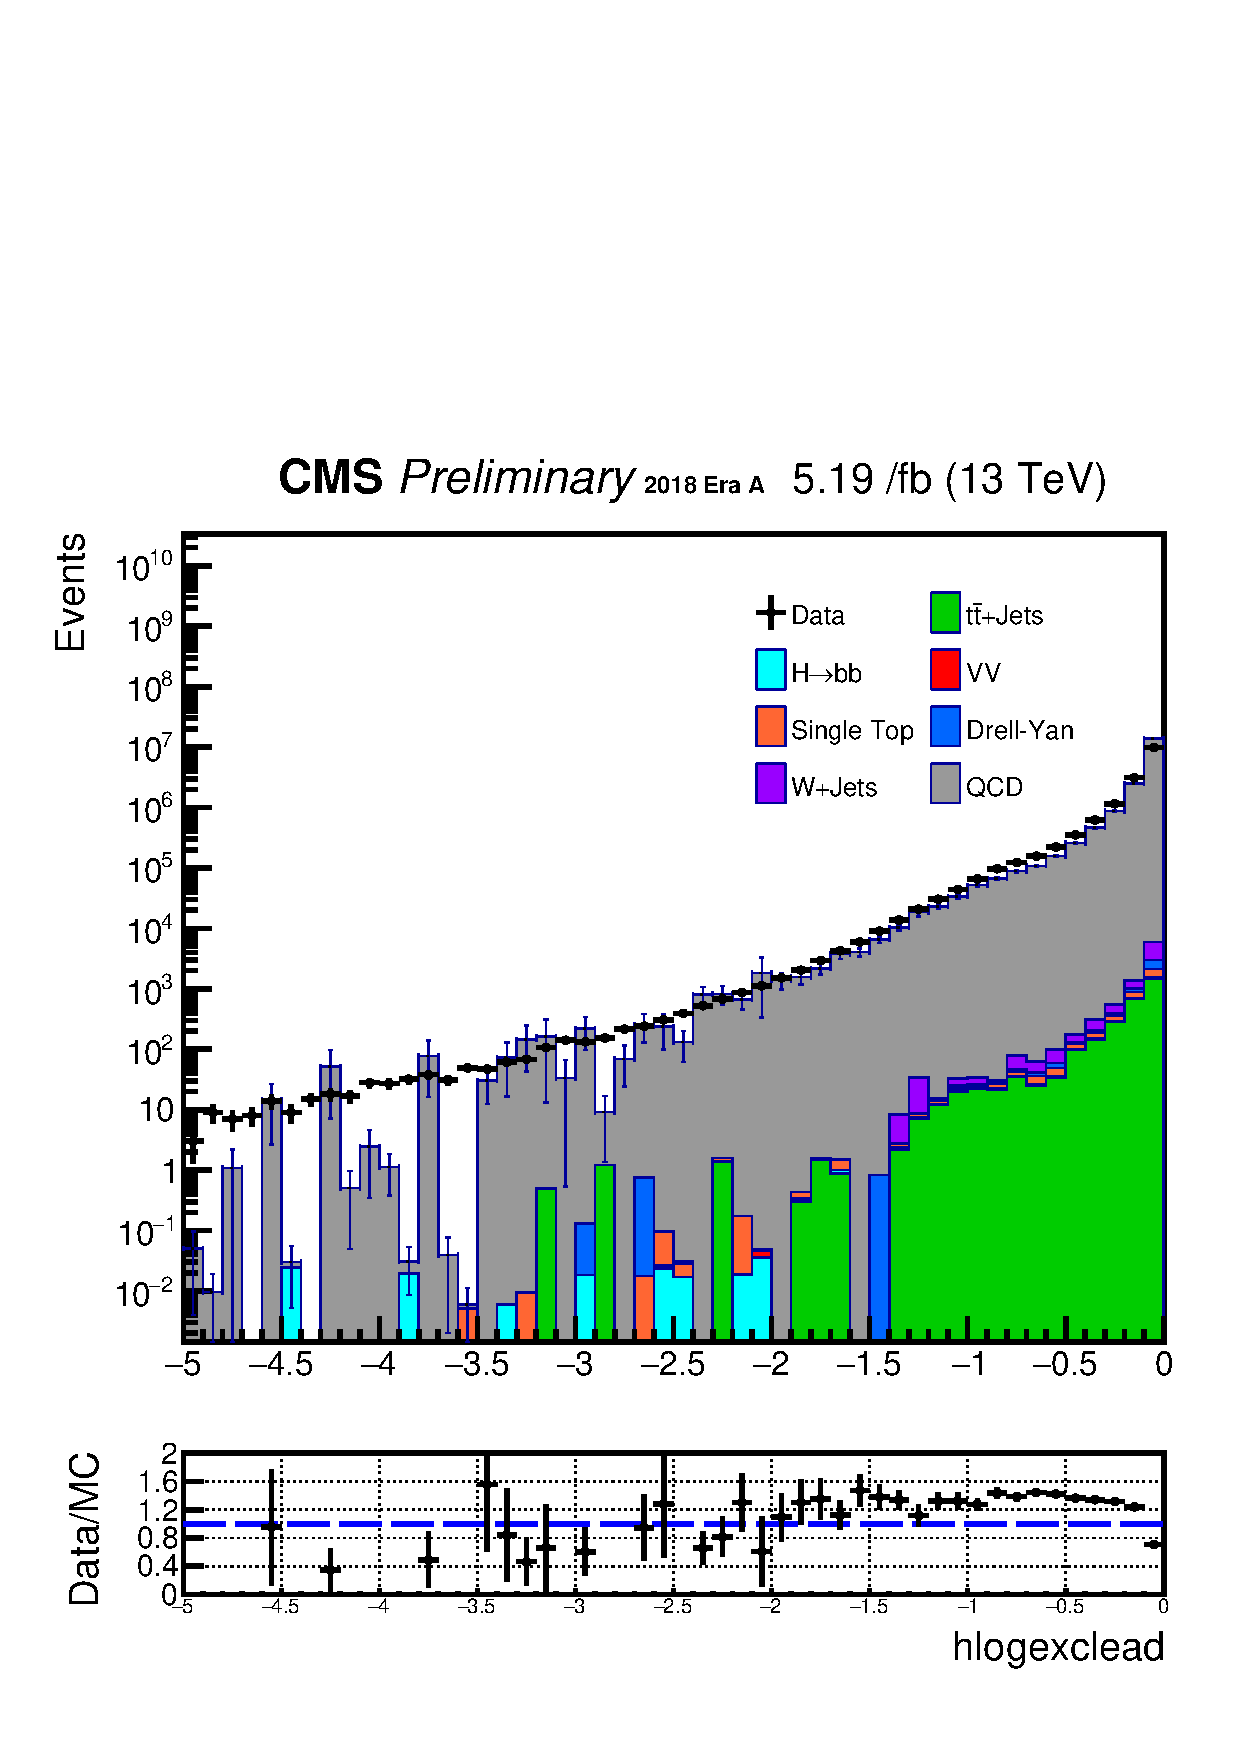
\includegraphics[width=0.40\linewidth]{figs/Data_log_Oct6ANVars_MS-15_ctauS-10_hlogexclead.pdf}
  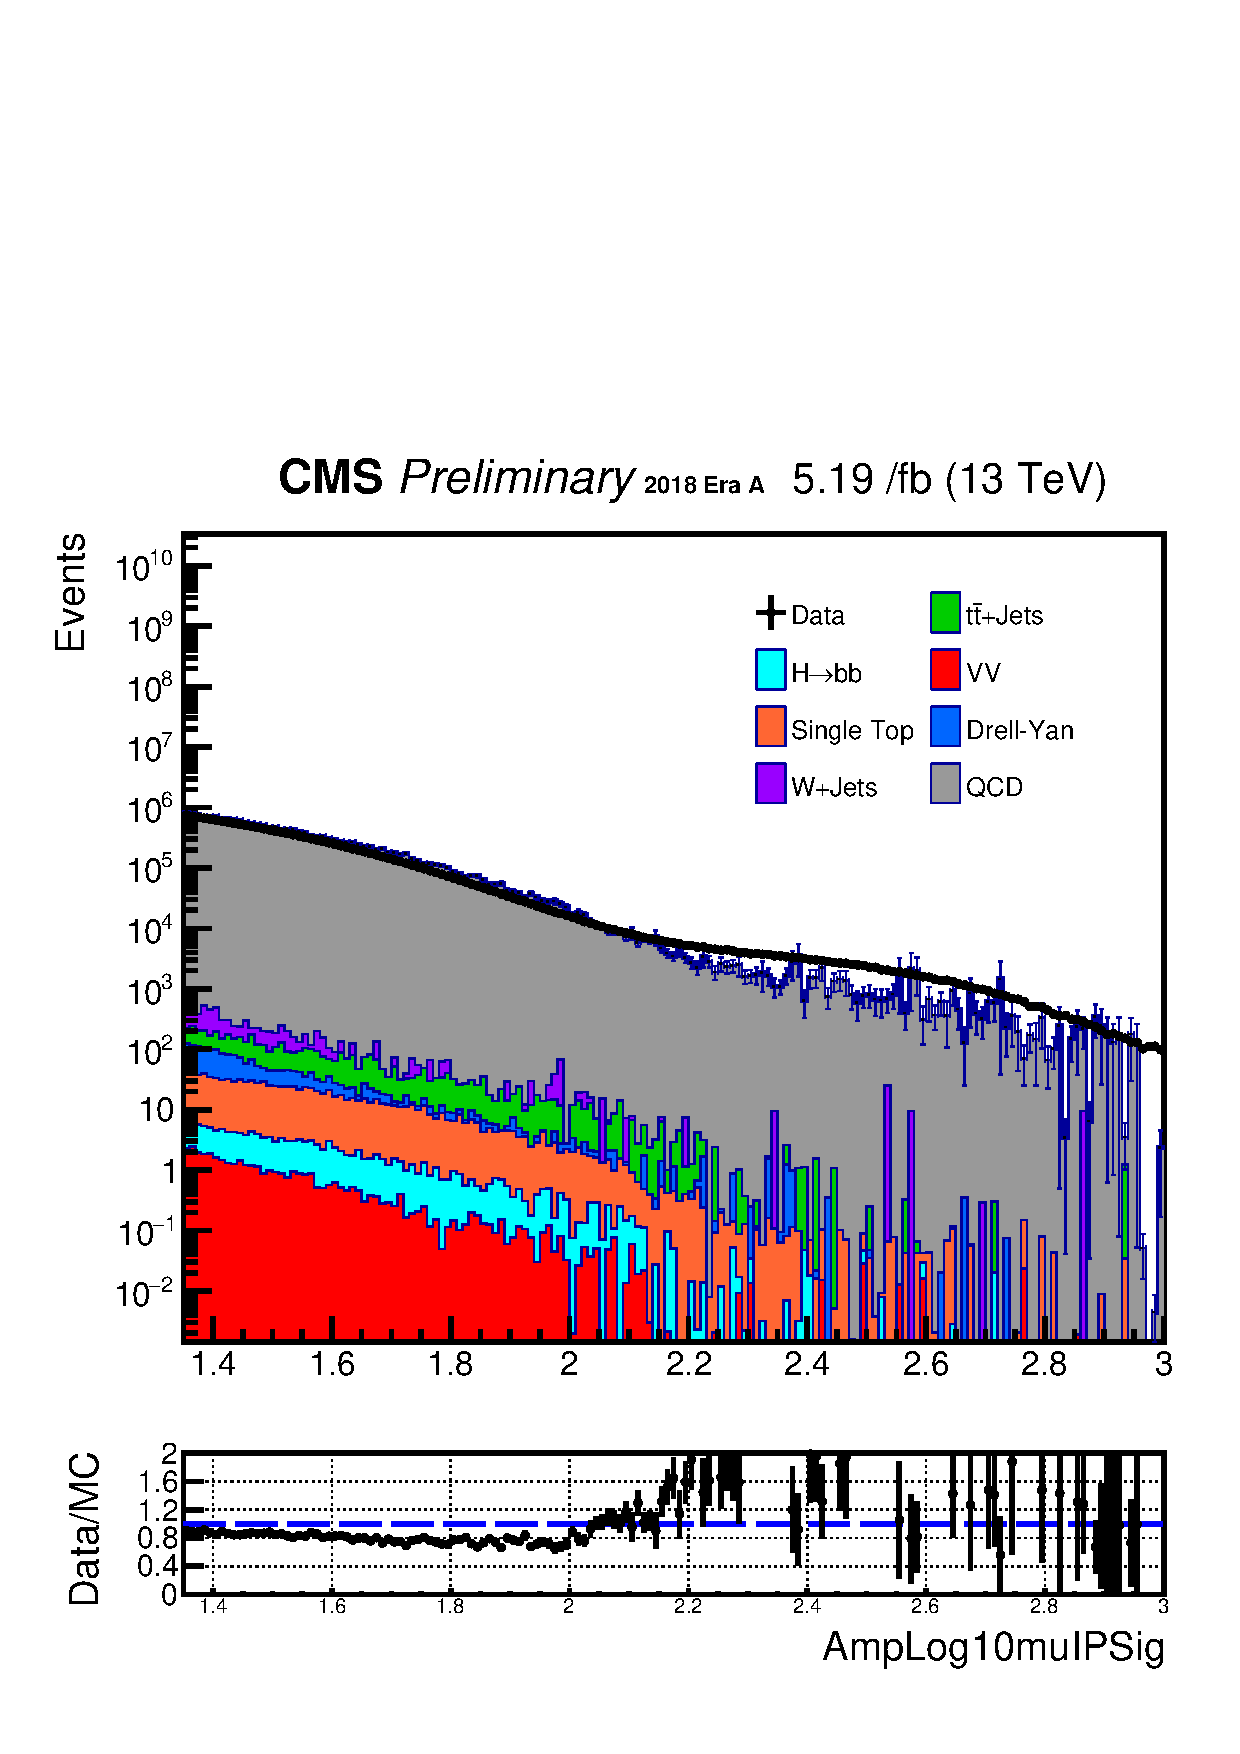
\includegraphics[width=0.40\linewidth]{figs/Data_log_Oct6ANVars_MS-15_ctauS-10_AmpLog10muIPSig.pdf}
	\caption{Data/MC agreement for distributions. High ROI scores and high Log10(muIPSig) values lack MC statistics}

\end{figure}
Section ~\ref{sec:selections} listed several different discriminant variables for the analysis.
Leading ROI vertex score, subleading ROI vertex score, and leading muon's IP value have the most discriminatory power.
Although the background MC samples describe the data's distribution reasonably well, one can also see discrepancies at higher vertex scores and IPSig values.
The discrepancy originates from 2 different reasons.
First, the lack of statistics is a fundamental deficiency for the MC samples.
Unlike 11.9 billion b-parking data events, MC sample events are simulated with extremely intensive computing resources.
Thus, its event number is below 100 million at most, failing to describe distributions for extreme values.
Second, the QCD MC's data description accuracy is lacking compared to other physics processes.
QCD background, the main background for the analysis, is a quantum-chromodynamics process.
QCD involves much uncertainty and relies on probabilistic description at low energy.
Therefore, QCD's description accuracy is lacking compared to other processes, such as WJets and the Drell-Yan process.
Since MC does not adequately describe the data, the analysis uses data-driven background estimation method.




\section{ABCD method}
ABCD method is the most preferred option for any background estimation method thanks to its simplicity.
ABCD method is the simplest form of transfer factor.
A ratio of background events at two control regions (CR) is applied to another CR's background event to infer background events in signal regions (SR) without unblinding.
The simplest mathematical for is described in formula \ref{eq:ABCD}.
\begin{equation}
\label{eq:ABCD}
	SR:CR1=CR2:CR3, SR=CR1*\frac{CR2}{CR3} 
\end{equation}

ABCD method requires two variables used for its estimation to be independent of each other for the background process.


Unfortunately, leading ROI and subleading ROI vertex scores are correlated in the QCD background process.
ROIs from B-mesons score higher in our TensorFlow.
In QCD processes, the B-mesons are likely to be pair produced.
Therefore, when the leading ROI vertex score is high due to a B-meson, the subleading ROI vertex score is also high because the other meson is produced at the same time.
Thus, due to their correlation, leading and subleading scores cannot be our ABCD discriminant variable candidates.

The analysis selects leading ROI and leading muon's IP value as its ABCD discriminant variables.
After implementing all other cuts (sublead ROI, $\Delta\Phi(lead,sublead)$, Annulus score, 1 Isolated $\mu$, $\Delta R(lead ROI, Jet)$), we tested the correlation factor between the leading ROI, and leading mu's IPSig values for each background process.
The values are pretty minimal except for 2-3 processes where there were too few entries to derive a solid conclusion due to statistical limitations.
%Therefore, the analysis uses leading Log10(IPSig) and leading ROI vertex score for its ABCD discriminant variables.
 \begin{figure}[h!]
   \label{fig:ABmethod}
   \centering
   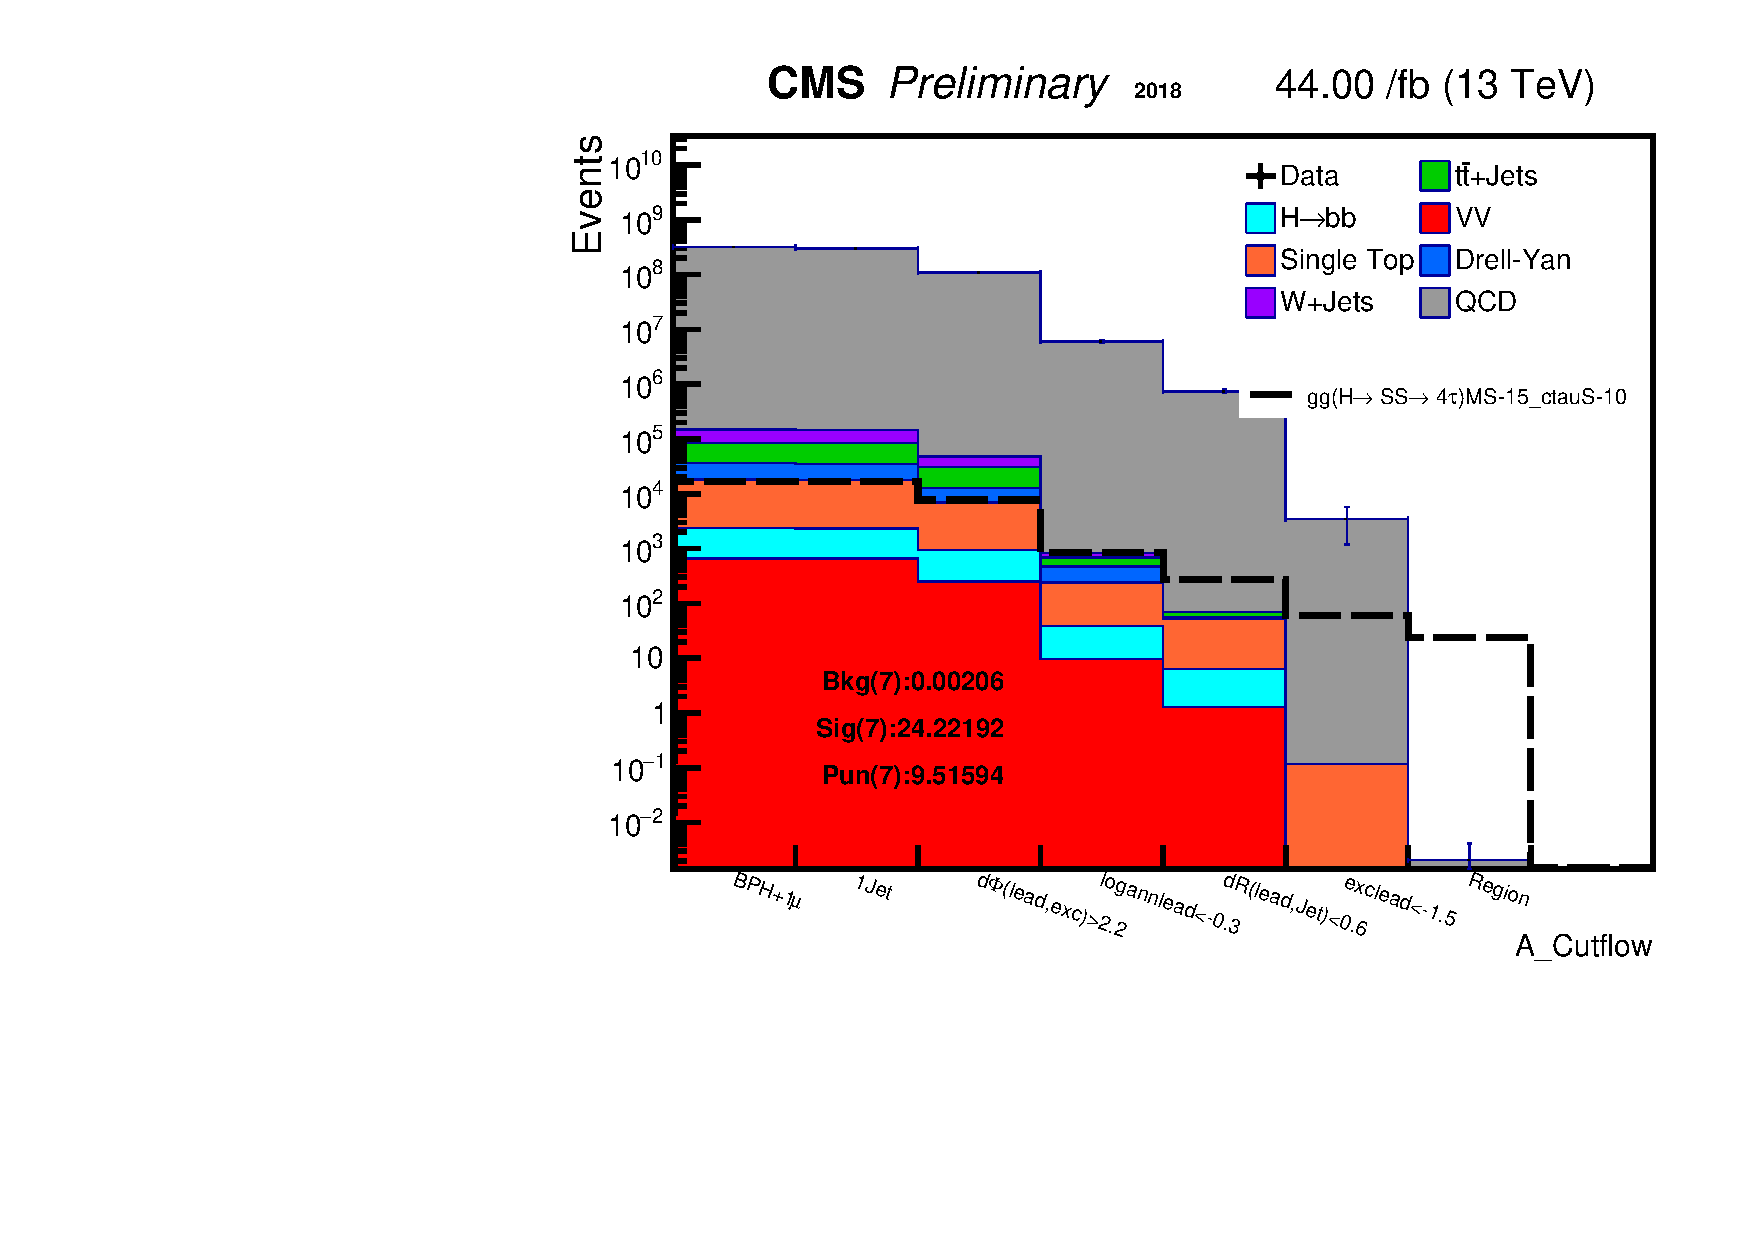
\includegraphics[width=0.47\linewidth]{figs/log_Oct6CutflAnalysisNote_MS-15_ctauS-10_A_Cutflow.pdf}
   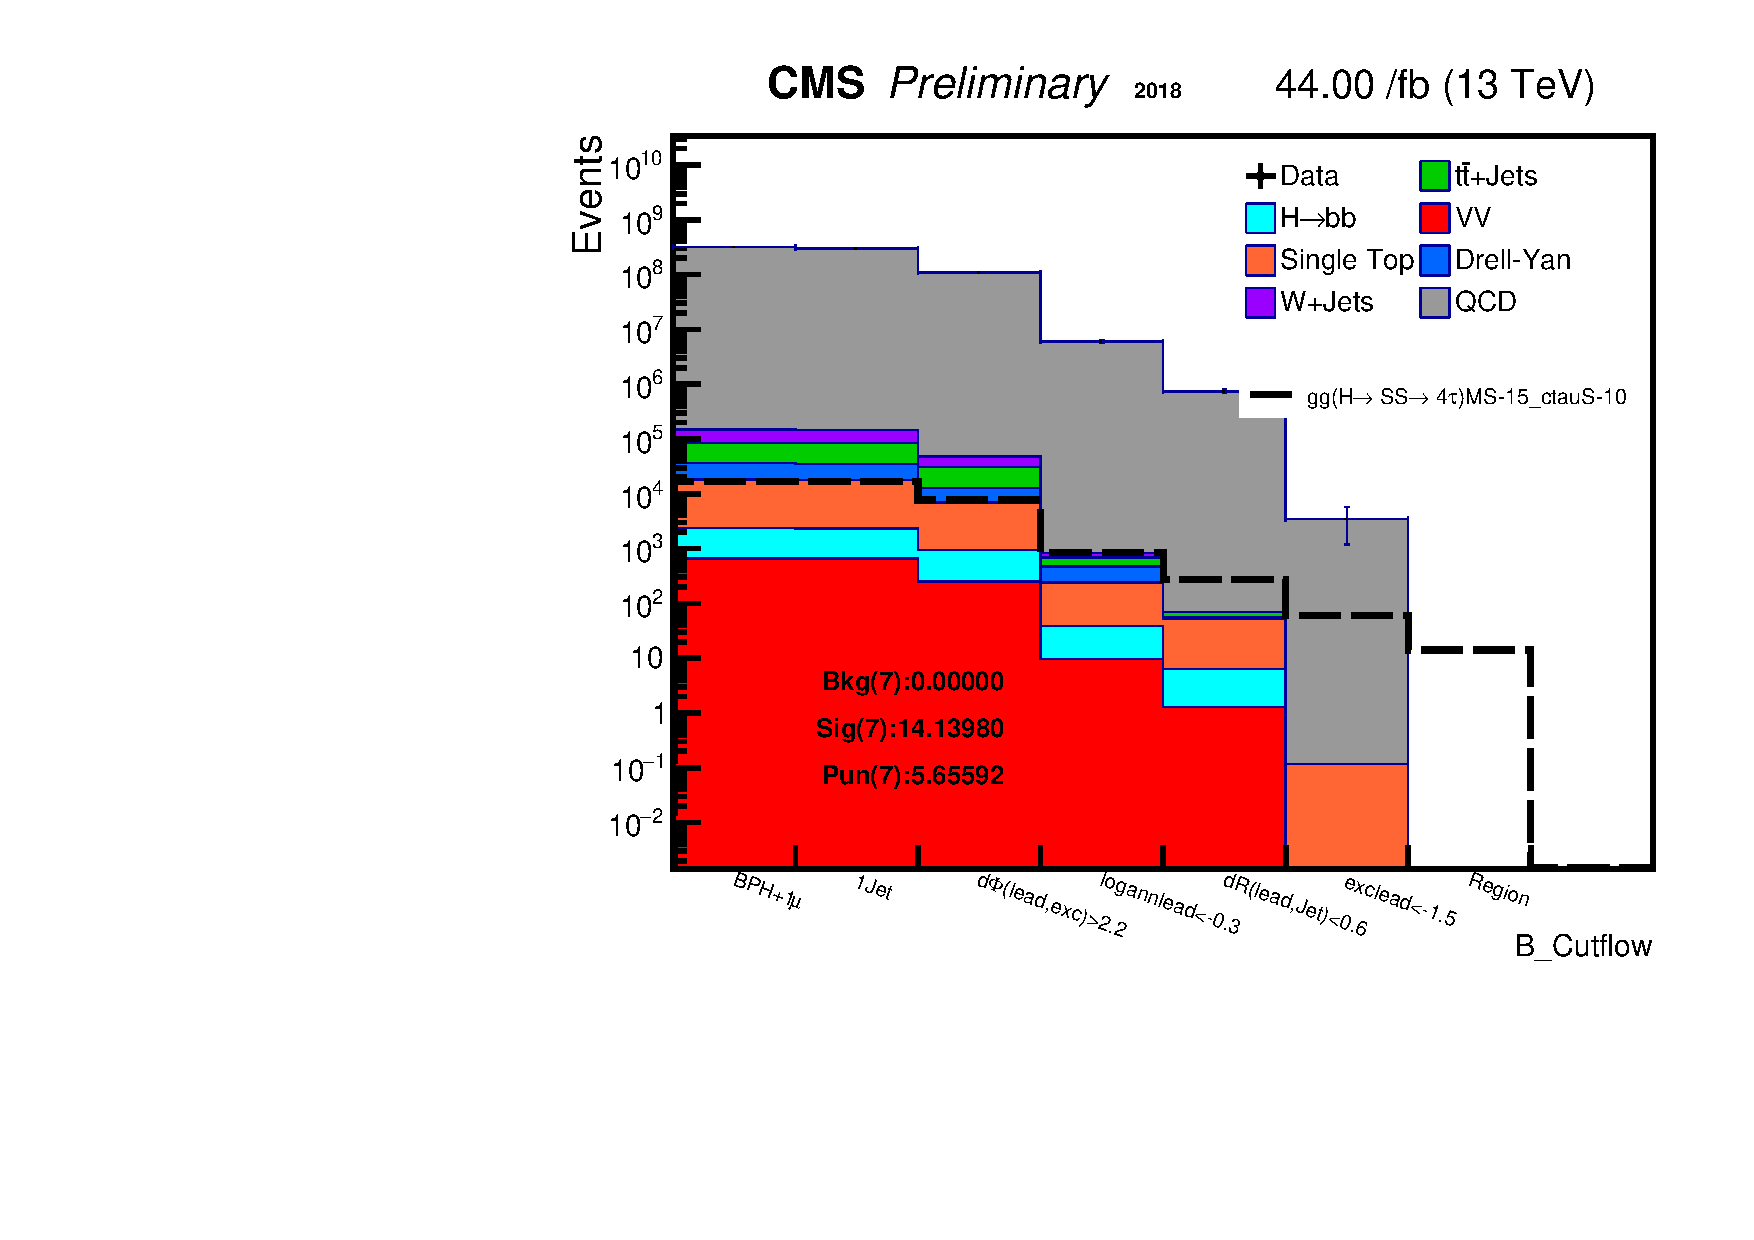
\includegraphics[width=0.47\linewidth]{figs/log_Oct6CutflAnalysisNote_MS-15_ctauS-10_B_Cutflow.pdf}
   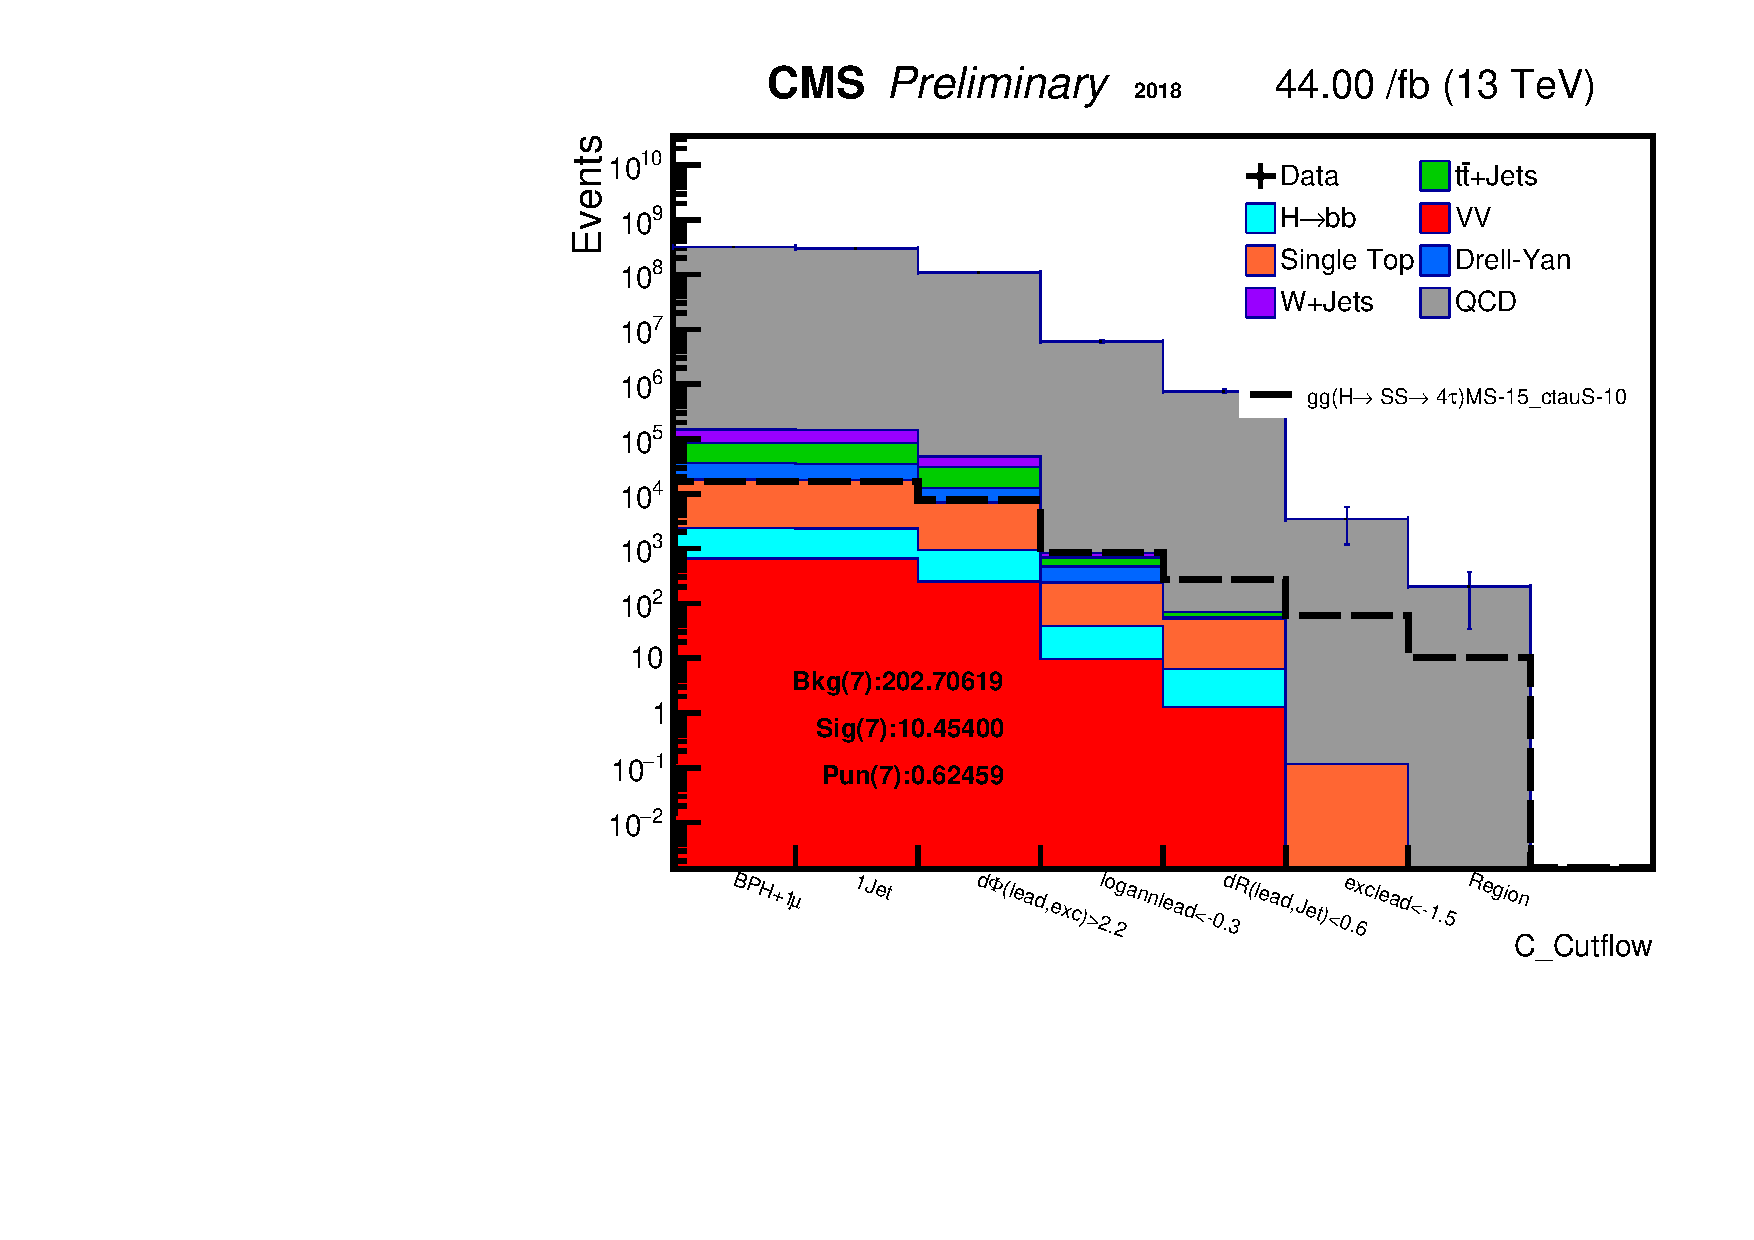
\includegraphics[width=0.47\linewidth]{figs/log_Oct6CutflAnalysisNote_MS-15_ctauS-10_C_Cutflow.pdf}
   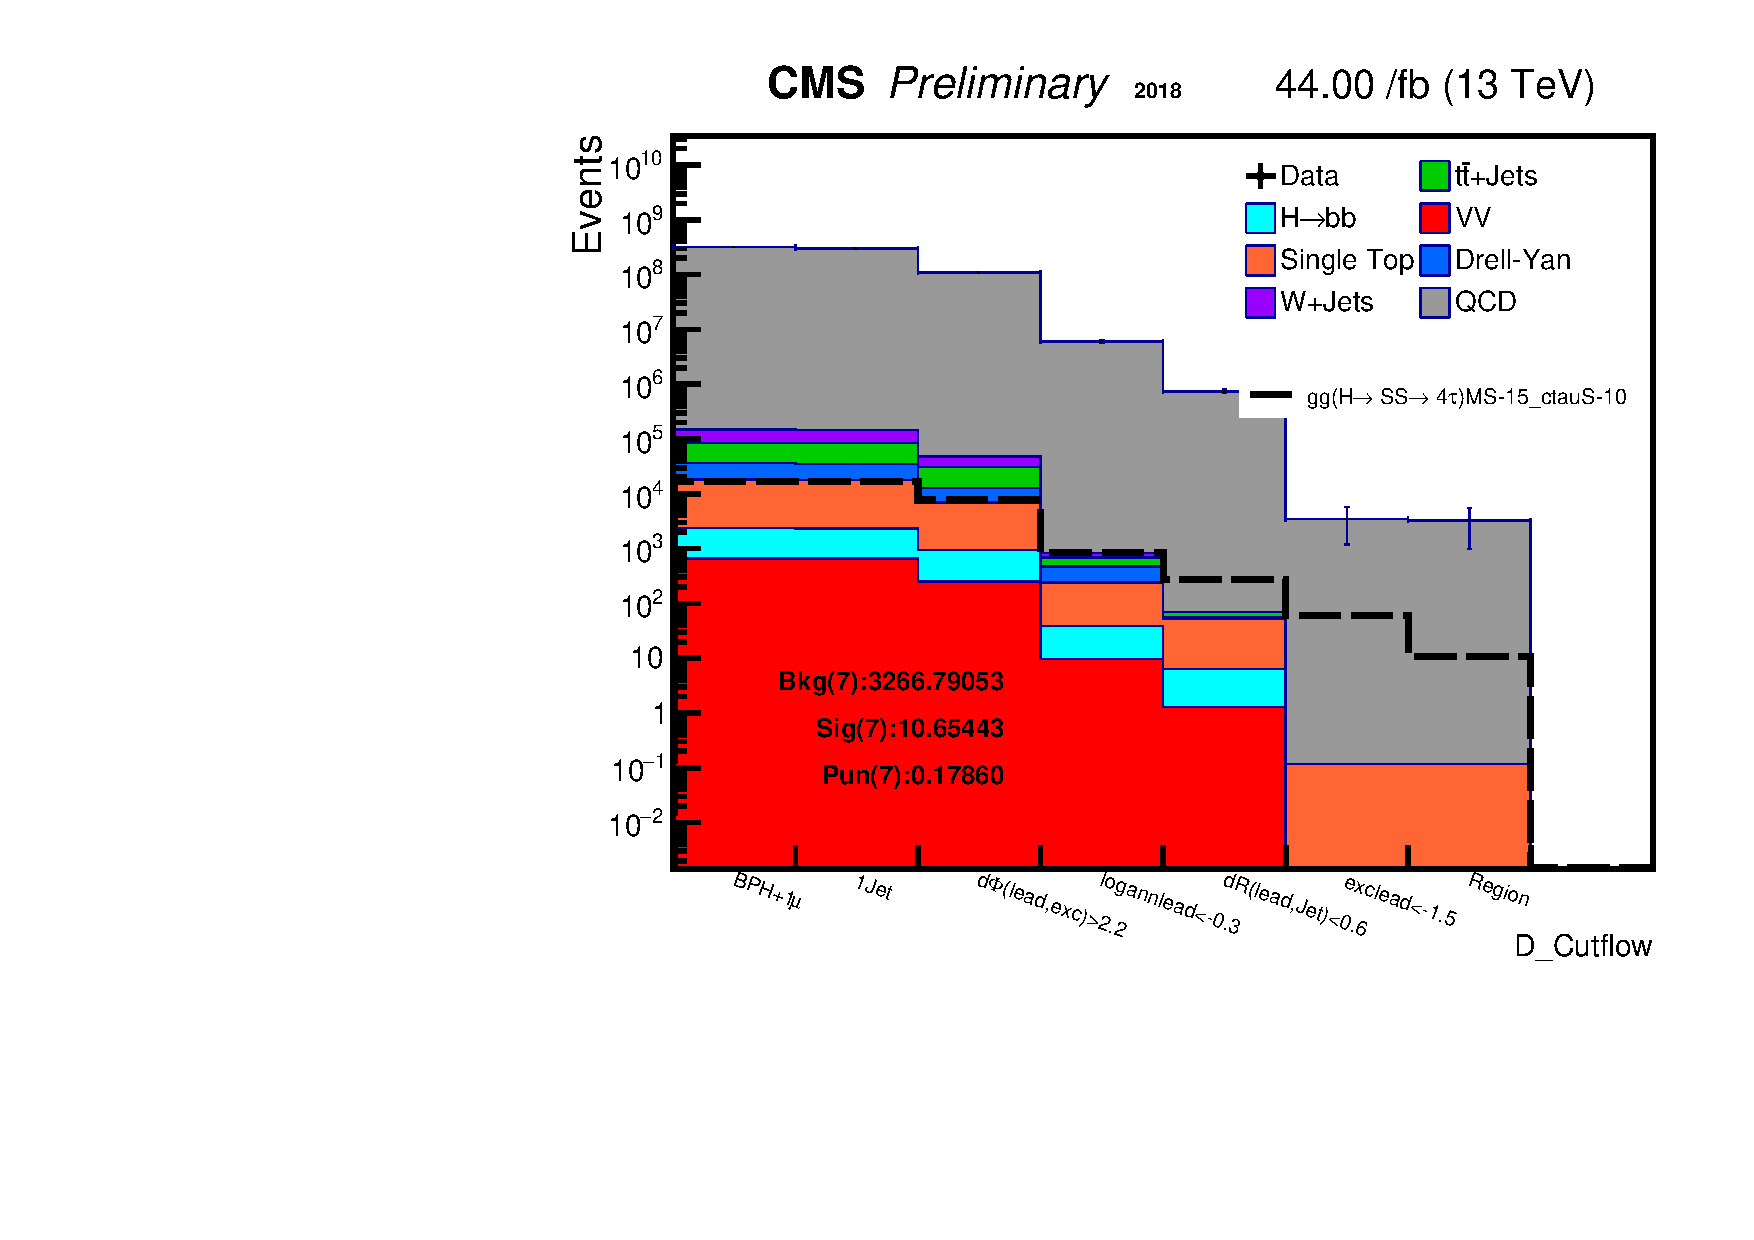
\includegraphics[width=0.47\linewidth]{figs/log_Oct6CutflAnalysisNote_MS-15_ctauS-10_D_Cutflow.pdf}
   \caption{Cutflow histogram of Signal versus background. The signal is MS15\GeV-ct10mm point. Last bin of the cutflow histogram is ABCD region selection. Top left plot is for region A, whereas the bottom right plot is for region D}
 \end{figure}

% \begin{figure}[h!]
%   \caption{Cutflow histogram of MS55GeV-ct10mm point. Left plot is for region A, whereas the right plot is for region D}
%   \label{fig:ABmethod2}
%   \centering
%   \includegraphics[width=0.47\linewidth]{figs/log_CutflAnalysisNote_MS-55_ctauS-10_A_Cutflow.pdf}
%   \includegraphics[width=0.47\linewidth]{figs/log_CutflAnalysisNote_MS-55_ctauS-10_B_Cutflow.pdf}
%   \includegraphics[width=0.47\linewidth]{figs/log_CutflAnalysisNote_MS-55_ctauS-10_C_Cutflow.pdf}
%   \includegraphics[width=0.47\linewidth]{figs/log_CutflAnalysisNote_MS-55_ctauS-10_D_Cutflow.pdf}
% \end{figure}
 \begin{figure}[h!]
   \label{fig:Finalbin}
   \centering
   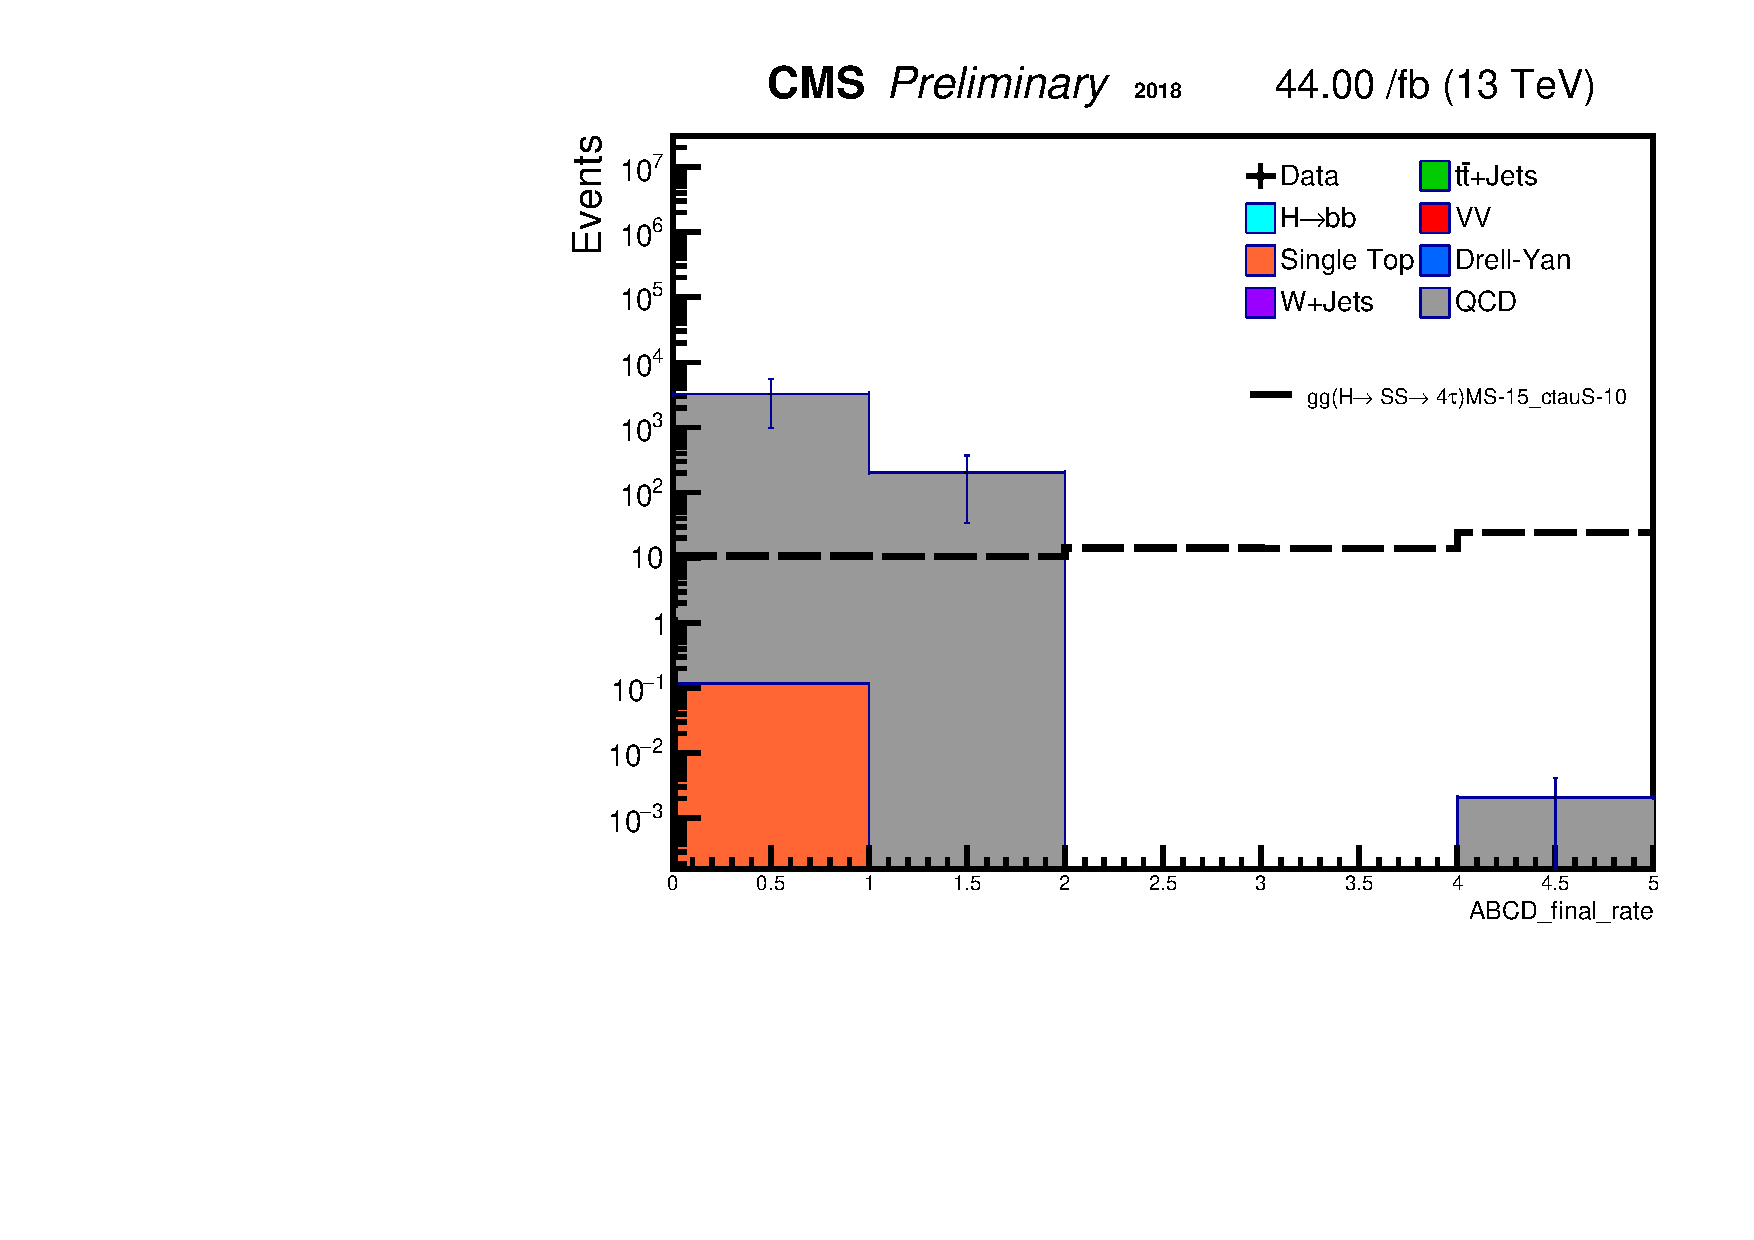
\includegraphics[width=0.67\linewidth]{figs/log_Oct6CutflAnalysisNote_MS-15_ctauS-10_ABCD_final_rate.pdf}
   \caption{Final bin of cutflow}
 \end{figure}



\begin{landscape}
\begin{table}[htb]
\caption{Region A's cutflow histogram by bin entry (weighted)}

\begin{tabular}{rllllllll}

 \hline 
&BPH+1mu & 1Jet & dPhi(lead,sub) & logannlead & dR(lead,Jet) & sublead & Region \\
 \hline 
 \hline 
MS15\GeV c$\uptau$ 10mm &1.6854e+04&1.6841e+04&7.7175e+03&8.5419e+02&2.7683e+02&5.9470e+01&2.4222e+01\\
 \hline 
TotBkgHist&3.1907e+08&2.9827e+08&1.1018e+08&6.0251e+06&7.4162e+05&3.4695e+03&2.0616e-03\\
 \hline 
QCD-Pt-15to20&4.5618e+07&4.0658e+07&1.3980e+07&1.1258e+06&6.0823e+04&0.0000e+00&0.0000e+00\\
 \hline 
QCD-Pt-20to30&1.1366e+08&1.0529e+08&3.8168e+07&2.1684e+06&2.2104e+05&0.0000e+00&0.0000e+00\\
 \hline 
QCD-Pt-30to50&1.1632e+08&1.1025e+08&4.1278e+07&2.0473e+06&3.3234e+05&2.0504e+03&0.0000e+00\\
 \hline 
QCD-Pt-50to80&3.4997e+07&3.3757e+07&1.3312e+07&5.3557e+05&9.7238e+04&1.1086e+03&0.0000e+00\\
 \hline 
QCD-Pt-80to120&6.9466e+06&6.8067e+06&2.8163e+06&1.1089e+05&2.1125e+04&2.8541e+02&0.0000e+00\\
 \hline 
QCD-Pt-120to170&9.8312e+05&9.7707e+05&4.1147e+05&2.9160e+04&7.0735e+03&6.3799e+00&0.0000e+00\\
 \hline 
QCD-Pt-170to300&3.6131e+05&3.5851e+05&1.5924e+05&6.6890e+03&1.7730e+03&1.6482e+01&0.0000e+00\\
 \hline 
QCD-Pt-300to470&2.2089e+04&2.2052e+04&1.0082e+04&3.9742e+02&1.2324e+02&1.8960e+00&0.0000e+00\\
 \hline 
QCD-Pt-470to600&1.5958e+03&1.5927e+03&7.4614e+02&2.7121e+01&9.9211e+00&1.2208e-01&0.0000e+00\\
 \hline 
QCD-Pt-600to800&5.8035e+02&5.7973e+02&2.7517e+02&8.3416e+00&3.7266e+00&6.3688e-03&0.0000e+00\\
 \hline 
QCD-Pt-800to1000&9.3006e+01&9.2944e+01&4.4374e+01&1.5118e+00&7.9019e-01&2.3820e-03&2.0616e-03\\
 \hline 
QCD-Pt-1000toInf&2.5854e+01&2.5830e+01&1.2238e+01&3.5332e-01&1.7023e-01&7.8399e-03&0.0000e+00\\
 \hline 
WJetsToLNu&6.5196e+04&6.0905e+04&1.6914e+04&1.4396e+02&0.0000e+00&0.0000e+00&0.0000e+00 \\
 \hline 
DYJetsToLL-M-50&1.8101e+04&1.7297e+04&5.8069e+03&2.2737e+02&3.0498e+00&0.0000e+00&0.0000e+00 \\
 \hline 
TTJets&4.8794e+04&4.8736e+04&1.8003e+04&2.1718e+02&1.2788e+01&0.0000e+00&0.0000e+00\\
 \hline 
ST-t-channel-top-5f&4.3424e+03&4.2675e+03&1.6261e+03&6.4960e+01&2.2447e+01&0.0000e+00&0.0000e+00\\
 \hline 
ST-s-channel-4f-leptonDecays&1.0063e+04&9.8535e+03&3.8657e+03&1.1469e+02&1.8001e+01&0.0000e+00&0.0000e+00\\
 \hline 
ST-tW-top&1.4277e+03&1.4234e+03&5.3647e+02&2.1466e+01&6.6034e+00&1.1637e-01&0.0000e+00\\
 \hline 
WW&2.5191e+02&2.4836e+02&9.0591e+01&5.6034e+00&8.4678e-01&0.0000e+00&0.0000e+00\\
 \hline 
WZ&2.4202e+02&2.3858e+02&9.2235e+01&2.4949e+00&6.0096e-02&0.0000e+00&0.0000e+00\\
 \hline 
ZZ&1.7331e+02&1.6886e+02&6.7381e+01&1.4956e+00&3.8633e-01&0.0000e+00&0.0000e+00\\
 \hline 
GluGluHToBB&1.6967e+03&1.6652e+03&7.0197e+02&2.9198e+01&5.1113e+00&0.0000e+00&0.0000e+00\\
 \hline 
VVhist&6.6723e+02&6.5581e+02&2.5021e+02&9.5939e+00&1.2932e+00&0.0000e+00&0.0000e+00 \\
 \hline 
ggHbbhist&1.6967e+03&1.6652e+03&7.0197e+02&2.9198e+01&5.1113e+00&0.0000e+00&0.0000e+00 \\
 \hline 
SThist&1.5833e+04&1.5544e+04&6.0283e+03&2.0111e+02&4.7051e+01&1.1637e-01&0.0000e+00\\
 \hline 
DYhist&1.8101e+04&1.7297e+04&5.8069e+03&2.2737e+02&3.0498e+00&0.0000e+00&0.0000e+00\\
 \hline 
TThist&4.8794e+04&4.8736e+04&1.8003e+04&2.1718e+02&1.2788e+01&0.0000e+00&0.0000e+00\\
 \hline 
WJhist&6.5196e+04&6.0905e+04&1.6914e+04&1.4396e+02&0.0000e+00&0.0000e+00&0.0000e+00\\
 \hline 
QCDhist&3.1892e+08&2.9812e+08&1.1014e+08&6.0242e+06&7.4155e+05&3.4694e+03&2.0616e-03\\
\end{tabular}
\label{tab:cutfl}
\centering
\end{table}
\end{landscape}



\begin{landscape}
\begin{table}[htb]
\caption{Region A's cutflow histogram by bin event number}
\begin{tabular}{rllllllll}

 \hline 
&BPH+1mu & 1Jet & dPhi(lead,sub) & logannlead & dR(lead,Jet) & sublead & Region \\
 \hline 
 \hline 
SigHist&2.2694e+05&2.2681e+05&1.0352e+05&1.2648e+04&4.1410e+03&8.5500e+02&3.4200e+02\\
 \hline 
TotHist&5.3177e+05&5.2132e+05&2.1245e+05&1.0073e+04&2.3160e+03&2.3000e+01&1.0000e+00\\
 \hline 
QCD-Pt-15to20&2.7520e+03&2.5260e+03&8.6400e+02&7.0000e+01&4.0000e+00&0.0000e+00&0.0000e+00\\
 \hline 
QCD-Pt-20to30&4.8608e+04&4.5901e+04&1.6665e+04&1.0160e+03&1.0700e+02&0.0000e+00&0.0000e+00\\
 \hline 
QCD-Pt-30to50&9.0101e+04&8.6625e+04&3.2269e+04&1.7380e+03&2.7400e+02&1.0000e+00&0.0000e+00\\
 \hline 
QCD-Pt-50to80&6.8298e+04&6.6504e+04&2.5810e+04&1.1720e+03&2.1300e+02&3.0000e+00&0.0000e+00\\
 \hline 
QCD-Pt-80to120&6.5713e+04&6.4742e+04&2.6313e+04&1.1520e+03&2.1400e+02&3.0000e+00&0.0000e+00\\
 \hline 
QCD-Pt-120to170&2.3205e+04&2.3121e+04&9.5490e+03&8.6400e+02&2.1800e+02&1.0000e+00&0.0000e+00\\
 \hline 
QCD-Pt-170to300&6.8059e+04&6.7665e+04&2.9518e+04&1.2610e+03&3.3200e+02&2.0000e+00&0.0000e+00\\
 \hline 
QCD-Pt-300to470&3.8598e+04&3.8550e+04&1.7291e+04&7.0500e+02&2.1900e+02&4.0000e+00&0.0000e+00\\
 \hline 
QCD-Pt-470to600&1.4636e+04&1.4614e+04&6.6820e+03&2.6400e+02&1.0000e+02&1.0000e+00&0.0000e+00\\
 \hline 
QCD-Pt-600to800&1.5791e+04&1.5777e+04&7.3730e+03&2.4500e+02&1.0200e+02&1.0000e+00&0.0000e+00\\
 \hline 
QCD-Pt-800to1000&2.8626e+04&2.8612e+04&1.3489e+04&4.8500e+02&2.4900e+02&4.0000e+00&1.0000e+00\\
 \hline 
QCD-Pt-1000toInf&8.4270e+03&8.4220e+03&3.9280e+03&1.1800e+02&5.7000e+01&2.0000e+00&0.0000e+00\\
 \hline 
WJetsToLNu&6.9900e+02&6.7400e+02&2.0000e+02&1.0000e+01&0.0000e+00&0.0000e+00&0.0000e+00\\
 \hline 
DYJetsToLL-M-50&2.3600e+03&2.2800e+03&7.8300e+02&3.7000e+01&3.0000e+00&0.0000e+00&0.0000e+00\\
 \hline 
TTJets&1.0453e+04&1.0447e+04&3.9980e+03&1.7900e+02&6.3000e+01&0.0000e+00&0.0000e+00\\
 \hline 
ST-t-channel-top-5f&5.7510e+03&5.6790e+03&2.1330e+03&9.6000e+01&2.9000e+01&0.0000e+00&0.0000e+00\\
 \hline 
ST-s-channel-4f-leptonDecays&1.6739e+04&1.6465e+04&6.5460e+03&2.7700e+02&5.4000e+01&0.0000e+00&0.0000e+00\\
 \hline 
ST-tW-top&5.8810e+03&5.8680e+03&2.1960e+03&8.9000e+01&2.9000e+01&1.0000e+00&0.0000e+00\\
 \hline 
WW&8.9600e+02&8.8600e+02&3.1900e+02&1.7000e+01&3.0000e+00&0.0000e+00&0.0000e+00\\
 \hline 
WZ&1.1810e+03&1.1670e+03&4.4900e+02&1.7000e+01&2.0000e+00&0.0000e+00&0.0000e+00\\
 \hline 
ZZ&9.2200e+02&9.0500e+02&3.5600e+02&1.0000e+01&2.0000e+00&0.0000e+00&0.0000e+00\\
 \hline 
GluGluHToBB&1.4070e+04&1.3888e+04&5.7160e+03&2.5100e+02&4.2000e+01&0.0000e+00&0.0000e+00\\
 \hline 
WJhist&6.9900e+02&6.7400e+02&2.0000e+02&1.0000e+01&0.0000e+00&0.0000e+00&0.0000e+00\\
 \hline 
DYhist&2.3600e+03&2.2800e+03&7.8300e+02&3.7000e+01&3.0000e+00&0.0000e+00&0.0000e+00\\
 \hline 
VVhist&2.9990e+03&2.9580e+03&1.1240e+03&4.4000e+01&7.0000e+00&0.0000e+00&0.0000e+00\\
 \hline 
TThist&1.0453e+04&1.0447e+04&3.9980e+03&1.7900e+02&6.3000e+01&0.0000e+00&0.0000e+00\\
 \hline 
ggHbbhist&1.4070e+04&1.3888e+04&5.7160e+03&2.5100e+02&4.2000e+01&0.0000e+00&0.0000e+00\\
 \hline 
SThist&2.8371e+04&2.8012e+04&1.0875e+04&4.6200e+02&1.1200e+02&1.0000e+00&0.0000e+00\\
 \hline 
QCDhist&4.7281e+05&4.6306e+05&1.8975e+05&9.0900e+03&2.0890e+03&2.2000e+01&1.0000e+00\\
\end{tabular}
\label{tab:Unitcutfl}
\centering
\end{table}
\end{landscape}







\section{Validation of ABCD method}
Although background MC's correlation factor($\hat{r}$) values are small, we need to verify that the data's correlation factor is negligible since data will be used for our background estimation.
However, direct computation of $\hat{r}$(leadROI,Log10(muIPSig)) for data is problematic because CMS collaboration stipulates ``blinding.''
In general, a high signal ratio is expected in the signal region.
In order to avoid bias for discovery and to change their analysis strategy accordingly, CMS collaboration recommends physicists blind themselves from looking into data entry in the signal region until community acknowledgment is granted.
This concept is called ``blinding.''
Since one can not access data entry in the signal region, the data's correlation factor($\hat{r}$) can not be computed.
Therefore, one needs to find an alternative way to estimate data's $\hat{r}$(leadROI,Log10(muIPSig)) without unblinding data in the signal region.

\begin{table}[htb]
\centering
\begin{tabular}{|p{3cm}|p{1cm}|p{1cm}|p{1cm}|p{1cm}|}
\hline
Lifetime & MS7 & MS15&MS40&MS55 \\
\hline
1mm & N/A & 7.43 & 1.68 & .947   \\
\hline
10mm & 343.2 & 833.6 & 767.2 & 427.8  \\
\hline
100mm & 141.1& 538.4 & 1011 & \textcolor{red}{1155} \\
\hline
1000mm & 13.4 & 68.5 & 129.7  &  163.1  \\
\hline
\end{tabular}
\label{tab:sigcont}
\centering
\caption{c$\uptau$,MS vs Signal Contamination in A' (Bkg :108k)}
\end{table}
For this purpose, we define a new ABCD region, referred to as A'B'C'D'.
A'-D' region is an orthogonal plane to the original ABCD, where the $\Delta\Phi$(lead,exclead) category of the event selection is flipped while all other event selection cuts are removed.
Region A', a correspondent Signal region of the orthogonal plane, should be much lower in the signal ratio (background dominated): Only so, looking into data entry in A' is not problematic.
In table \ref{tab:sigcont}, we confirm that the background dominates the A' region while the signal is low regardless of the signal's MS and ctau.




\begin{figure}[h!]
  \label{fig:valcar}
  \centering
  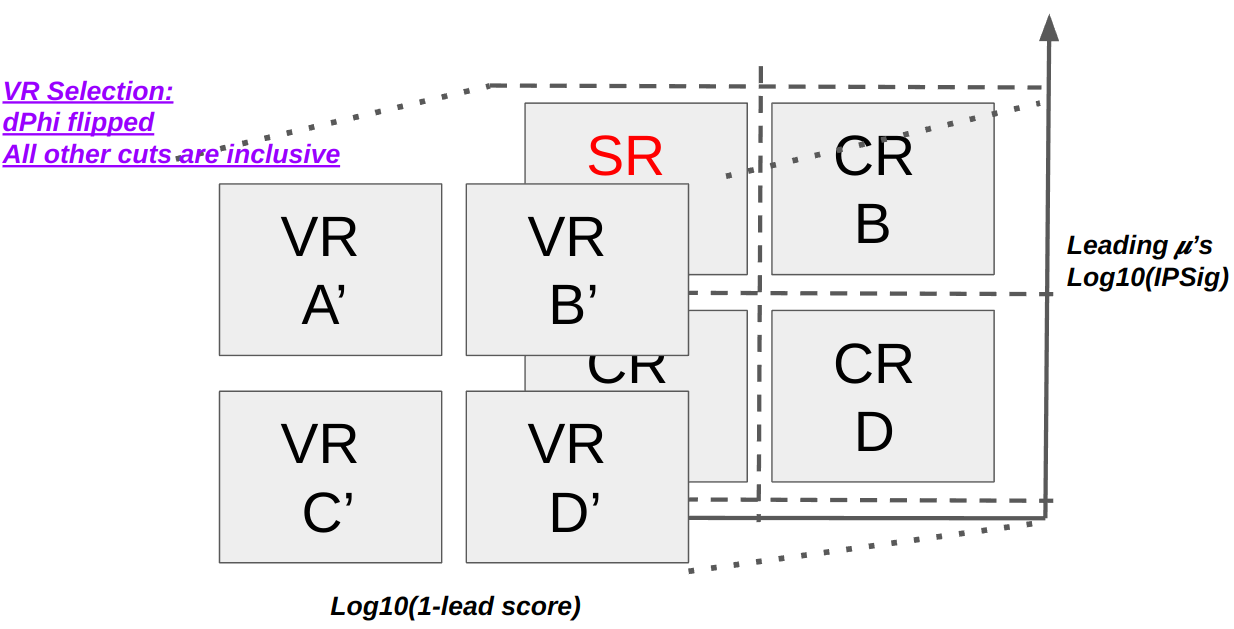
\includegraphics[width=0.85\linewidth]{figs/SimpleVR.png}
  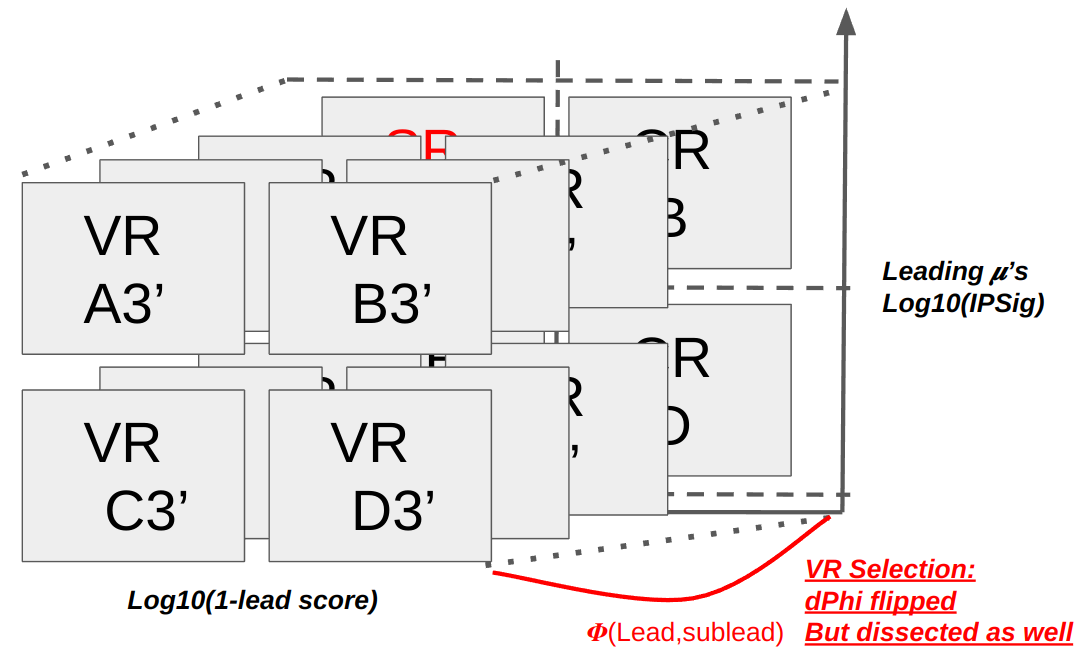
\includegraphics[width=0.85\linewidth]{figs/SophiVR.png}
  \caption{Cartoon description of ABCD method validation. The first figure shows a simpler definition of validation region. The second figure shows a more sophisiticated definition of validation regions. }

\end{figure}

\begin{figure}[h!]
  \label{fig:valcar}
  \centering
  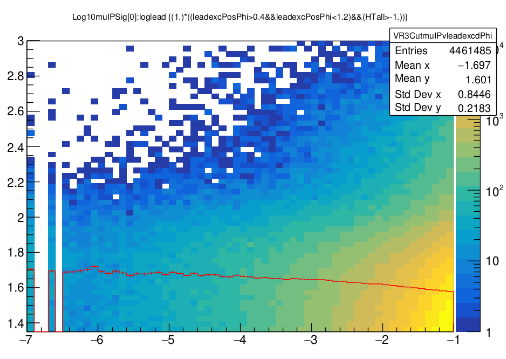
\includegraphics[width=0.65\linewidth]{figs/VR3.png}
	\caption{Profile plot of VR. Correlation factor is 0.105. ProfileX is rather flat. X-axis is log10(1-leading ROI score). Y-axis is Log10(muIPSig).}

\end{figure}


\begin{figure}[h!]
  \label{fig:valcar1}
  \centering
  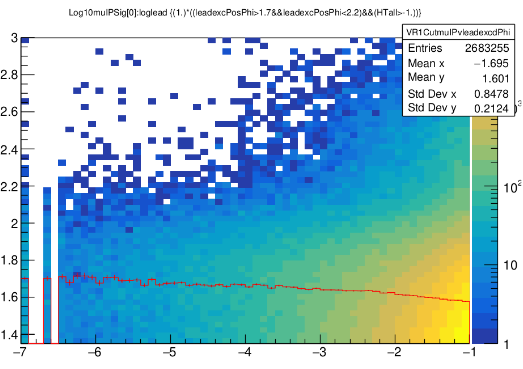
\includegraphics[width=0.65\linewidth]{figs/VR1.png}
  \caption{Profile plot of VR1. Correlation factor is 0.124. ProfileX is rather flat. X-axis is log10(1-leading ROI score). Y-axis is Log10(muIPSig).}

\end{figure}

\begin{figure}[h!]
  \label{fig:valcar2}
  \centering
  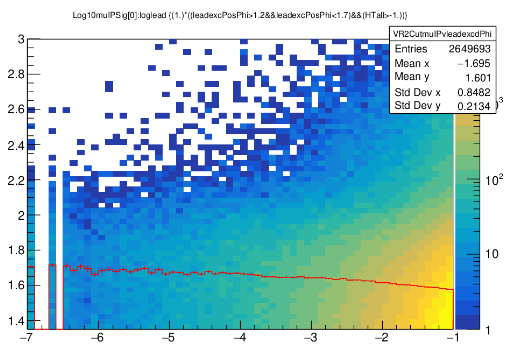
\includegraphics[width=0.65\linewidth]{figs/VR2.png}
  \caption{Profile plot of VR2. Correlation factor is 0.1229. ProfileX is rather flat. X-axis is log10(1-leading ROI score). Y-axis is Log10(muIPSig).}

\end{figure}

\begin{figure}[h!]
  \label{fig:valcar3}
  \centering
  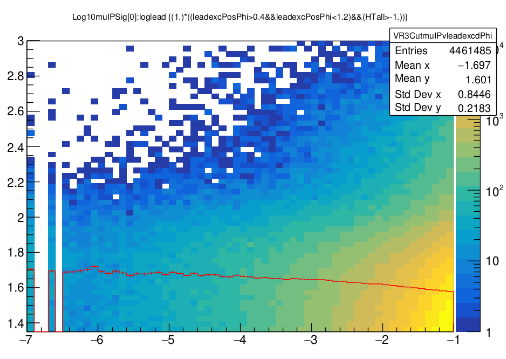
\includegraphics[width=0.65\linewidth]{figs/VR3.png}
  \caption{Profile plot of VR3. Correlation factor is 0.1203. ProfileX is rather flat. X-axis is log10(1-leading ROI score). Y-axis is Log10(muIPSig).}

\end{figure}


In figure \ref{fig:valcar}, we can see the correlation factor is small at about 10\%, still a negligible value.
With $\hat{r}$(leadROI,Log10(muIPSig)) value in A'-D' region, It seems sufficient to claim that there should be a negligible correlation between leadROI and Log10(muIPSig) for the A-D region as well.
However, We could have 1 more diagnostic question before unblinding.
What if $\hat{r}$(leadROI,Log10(muIPSig)) value changes with respect to $\Delta\Phi$(lead,exclead)?
If the formula in \ref{eq:rhat} is not true, \newline $\hat{r}$(leadROI,Log10(muIPSig)) obtained from A'-D' is not a good estimate for $\hat{r}$(leadROI,Log10(muIPSig)) for A-D.


\begin{equation}
\label{eq:rhat}
	\frac{d\hat{r}(leadROI,Log10(muIPSig))}{d\Delta\Phi(lead,exc)}=0
\end{equation}
We subdivide A'-D' to check that formula \ref{eq:rhat} is true.
A1'-D1' are orthogonal planes where $\Delta\Phi$(lead,exclead) is closest to A-D. 
Increasing numeric value indicates how far the $\Delta\Phi$(lead,exclead) is from the A-D. 
$\hat{r}$(leadROI,Log10(muIPSig)) value for each of A'-D' region is plotted and summarized in figures \ref{fig:valcar1}-\ref{fig:valcar3} .



As we scan $\hat{r}$(leadROI,Log10(muIPSig)) for each $\Delta\Phi$(lead,exclead) section, very small trend with respect to $\Delta\Phi$(lead,exclead) is observed.
We can claim the formula \ref{eq:rhat} is true and \newline $\hat{r}$(leadROI,Log10(muIPSig)) from A'-D' can be translated into A-D region as well.
Since there is little correlation between the two variables for the ABCD region, we validated the background estimation method.
With the background rate in the signal region estimated by the ABCD method with data, and with signal MC, we can claim whether there exists a signal over the SM expectation or not.
If it does not, we can set an exclusion limit on the Higgs branching ratio to our final state at a specific value.

Before that final step, systematic uncertainty is described in the following section for exclusion limit calculation.

